
\section{Experimental Apparatus}
The experiment was carried out at the Idaho Accelerator Center, using their short pulsed linear accelerator. The accelerator is a radio frequency accelerator operating at the L--band frequency of 1300 MHz. It is capable of pulse widths ranging from 50 ps to 2 $\mu$s with a maximum energy of 44 MeV.


\begin{figure}[h]
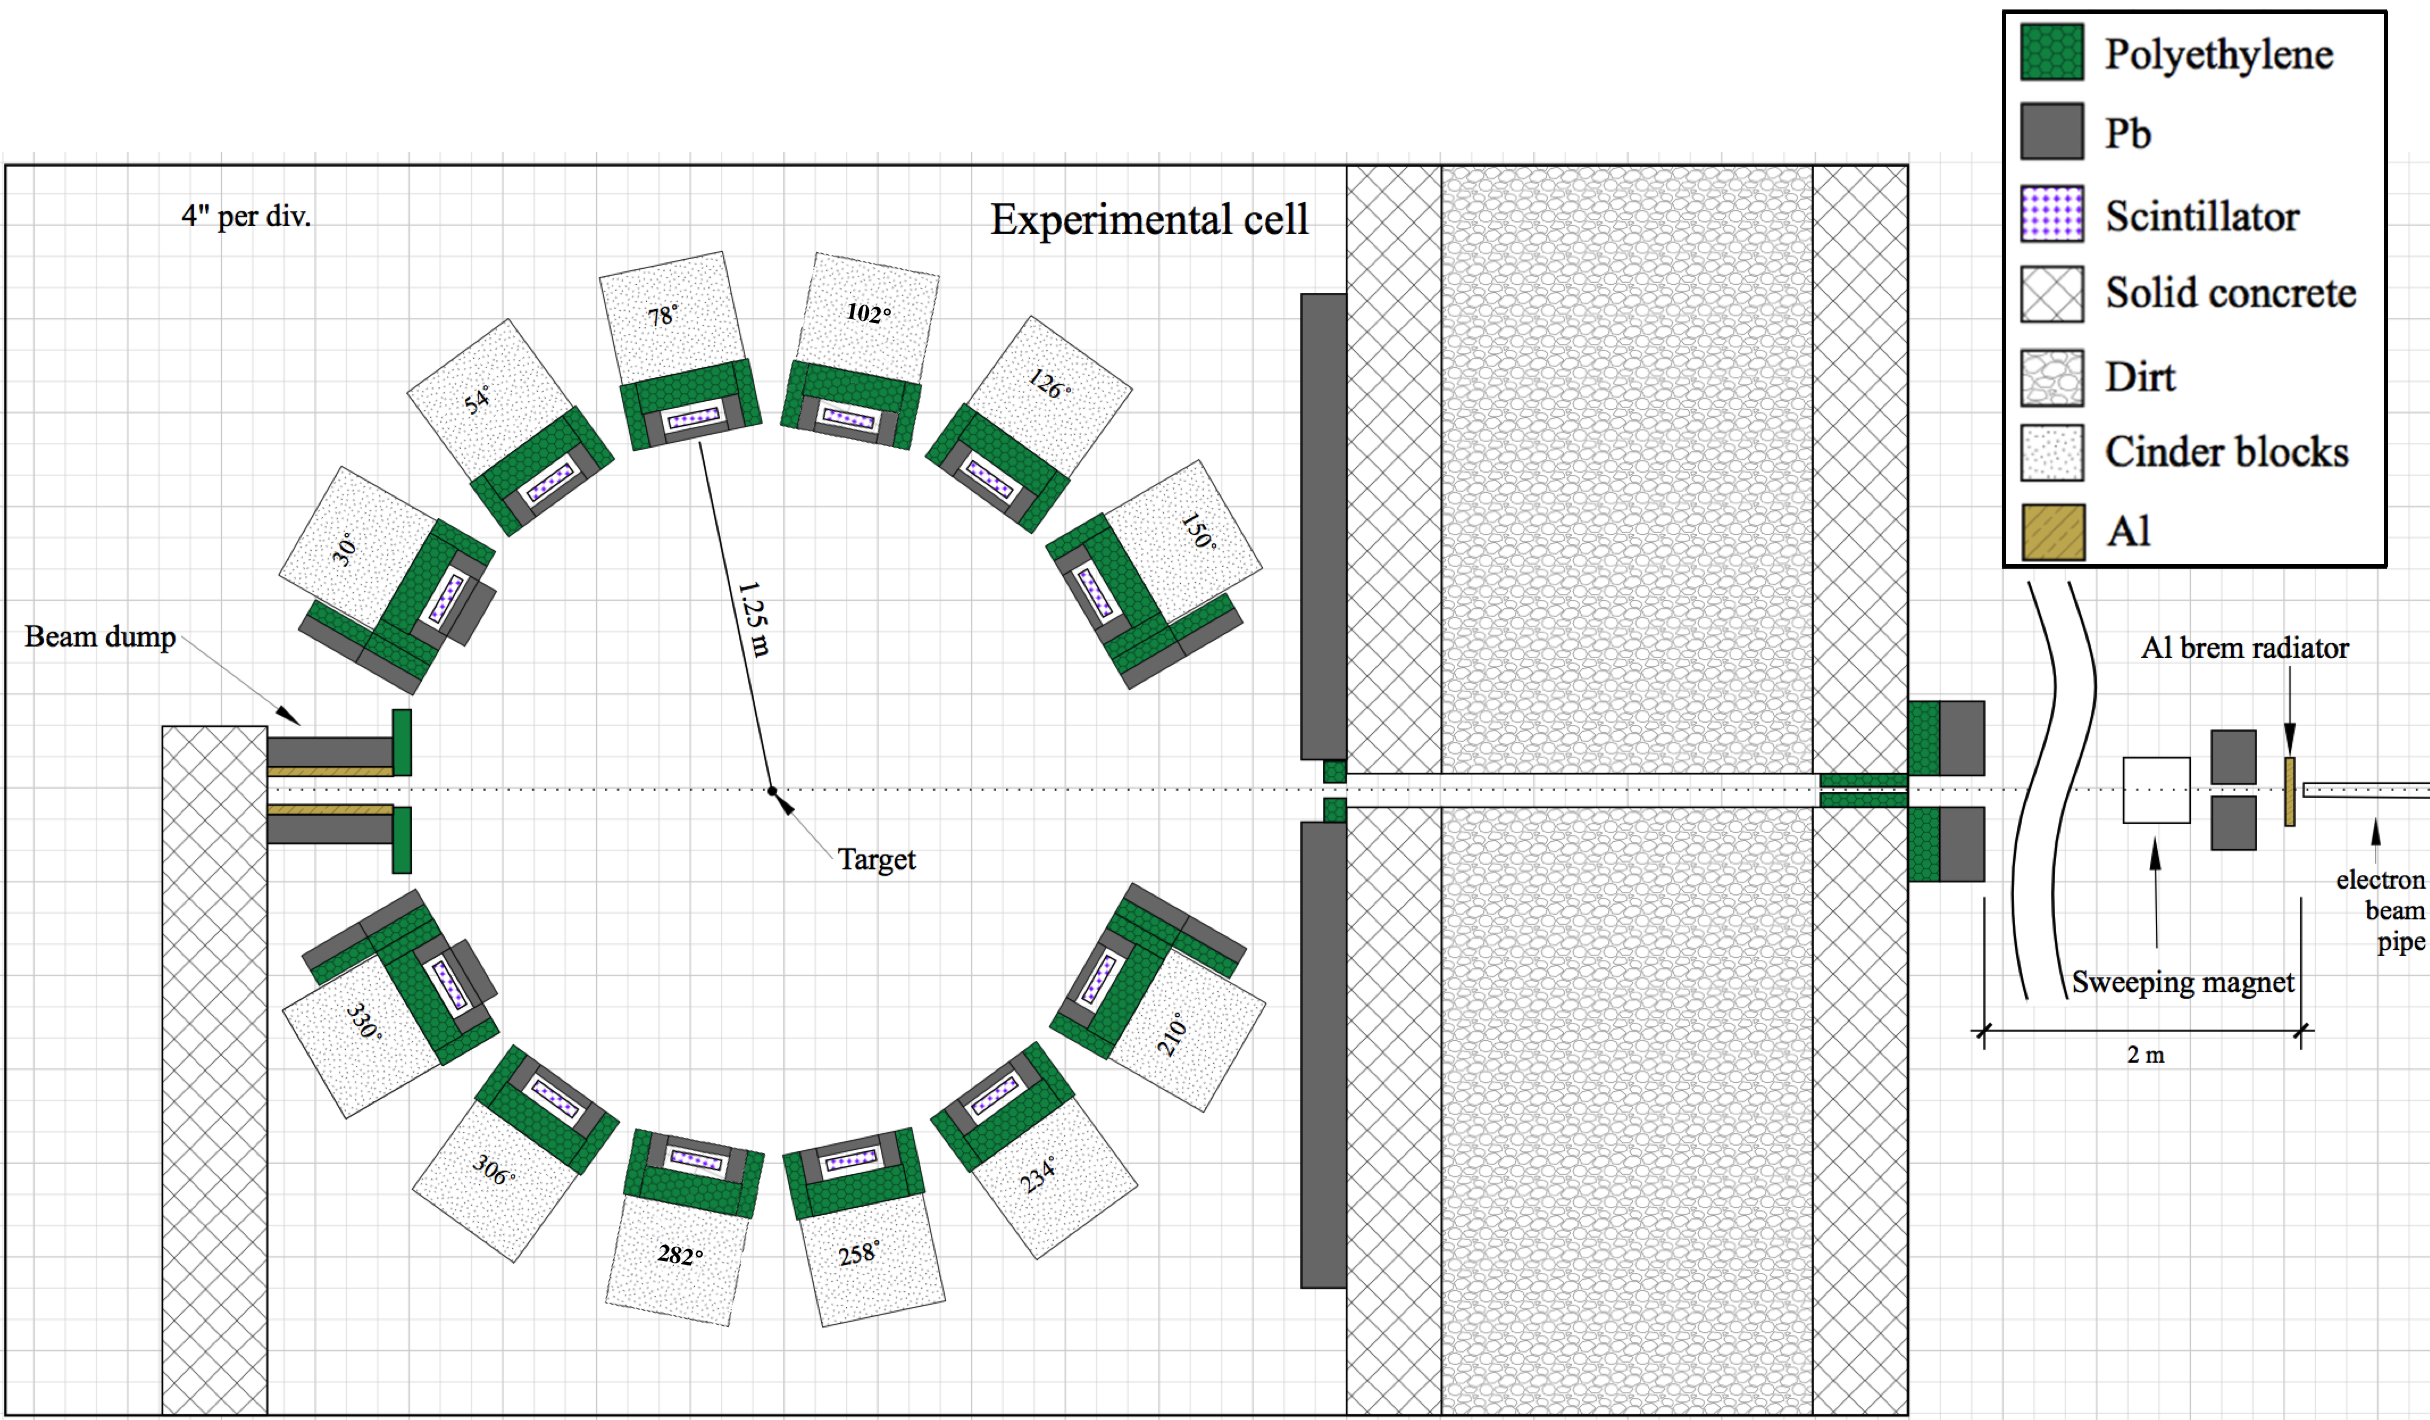
\includegraphics[width=\textwidth]{Content/Methods/ExpArangment.png}
\caption{To-scale top down schematic of the entire experimental setup.
The detectors supporting structures are each labeled with a degree value.
The degree corresponds to the angle of the detector from the direction of the beam.
For a better perspective of the scintillation cells alone, see ~\ref{fig:DetGeom}}
\label{fig:Facility}
\end{figure}

\subsection{Detectors}
\begin{figure}[h]
\centering
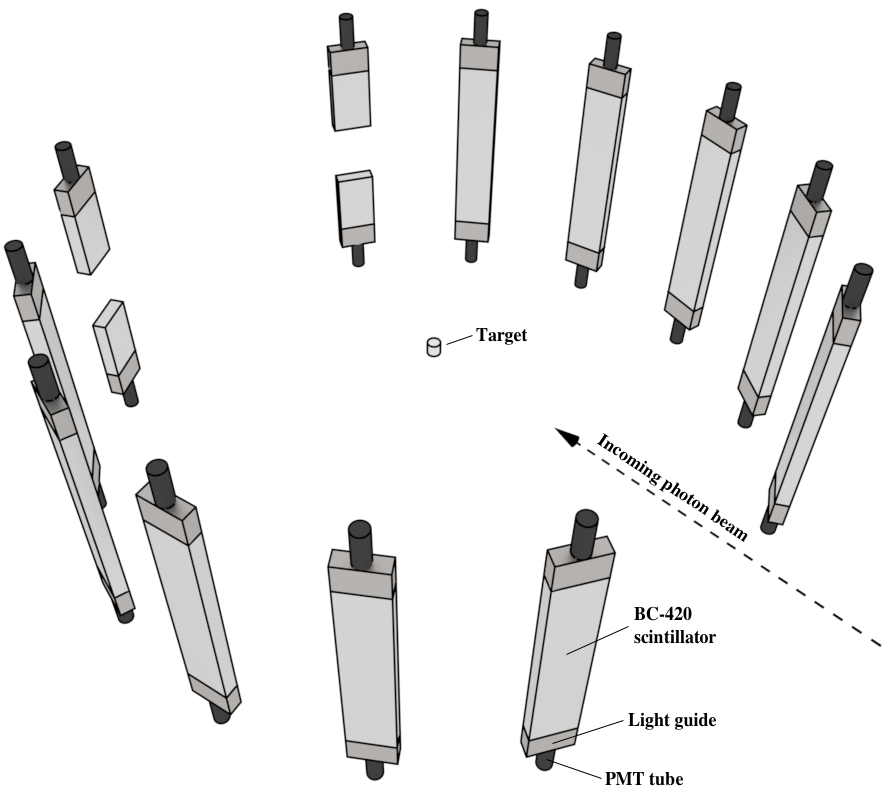
\includegraphics[width=0.95\textwidth]{Content/Methods/Detectors.png}
\caption{3D-rendering of the bare scintillation cells showing how the detectors are positioned in space.
Each detector is fully enclosed in a shielding structure, which is not shown in this depiction.}
\label{fig:DetGeom}
\end{figure}
The neutron detector array consists of fourteen cells made from BC-420 scintillation material acquired from the Transportation Security Administration (TSA) as surplus.
The scintillation cells were arranged in a ring around the target (see figure ~\ref{fig:DetGeom}).
The scintillators are instrumented with Hamamatsu 580-17 photomultiplier (PMT) tubes.
Two different detector designs had to be used in order to address a high rate of gammas on the detectors located furthest downstream of the beam.
Ten of the fourteen detectors did not have this problem, and have dimensions of 76.2X15.2X3.8 cm$^3$.
The remaining four had their dimensions reduced to 25.4X15.2X3.8 in order to address particularly rates of gamma detection, which are caused by the scattering of photons from the target.
This scattering of photons creates a cone of gammas that engulfs forward facing detectors, leading to very high levels of dead-time and an effective neutron efficiency of zero.
To counter this, the detectors at $\pm$30 degrees from the downstream beam line were reduced to 1/3 the size of the rest of the detectors and instrumented with only a single PMT.
Prior to this modification, the gamma detection rate per pulse nearly 1 in each of these detectors.
After the modification, the gamma detection rate fell to 0.5 gammas per pulse, leading to a net increase in the effective neutron detection efficiency.

The location of a particle hit along the detector's 30 inch length is determined by the timing difference between signals in the top and bottom PMT. This method uses the fact that the scintillation light travels at a constant speed through the cell. This technique is not possible for the four the downstream detectors at $\pm 30^{\circ}$, since these have only a single PMT. For these detectors, particle position is assumed to be at the middle of the cell. For further detail on particle position reconstruction, see section ~\ref{reconstruction}. 

In order prevent scintillation light from escaping the scintillators, they were wrapped in reflective Tyvek. This increases efficiency by facilitating the propagation of light between the point of scintillation and the PMTs. As a further measure to contain scintillation light, the cells were buffered with a (what?), which removes micro imperfections that could allow light to escape. If the cell is perfectly smooth, then light that is incident on the inner surface will be reflected back into the cell, because detector geometry will ensure that the light's angle of incidence with the cell's surface is below the angle of total internal reflection. 

\subsection{Data Acquisition}
A data acquisition system based on NIM/VME standard was used. A wiring diagram is shown in figure~\ref{fig:WiringDiagram}. The PMTs are supplied voltages ranging from 1300 to 1500 V by a Locroy 1458 high voltage mainframe. The analogue signals from the PMTs are fed into a leading edge discriminator with input thresholds ranging from 30 mV to 50 mV. The logic signals from the discriminator are then converted to ECL logic and fed into a CAEN model V1290A TDC. A gun signal from the accelerator provided the “start” signal for each pulse.
On the software side, the acquisition of data from the TDC, along with the conversion of the data into usable formats, was carried out using the CODA software package developed by Jefferson Lab.  

\begin{figure}[h]
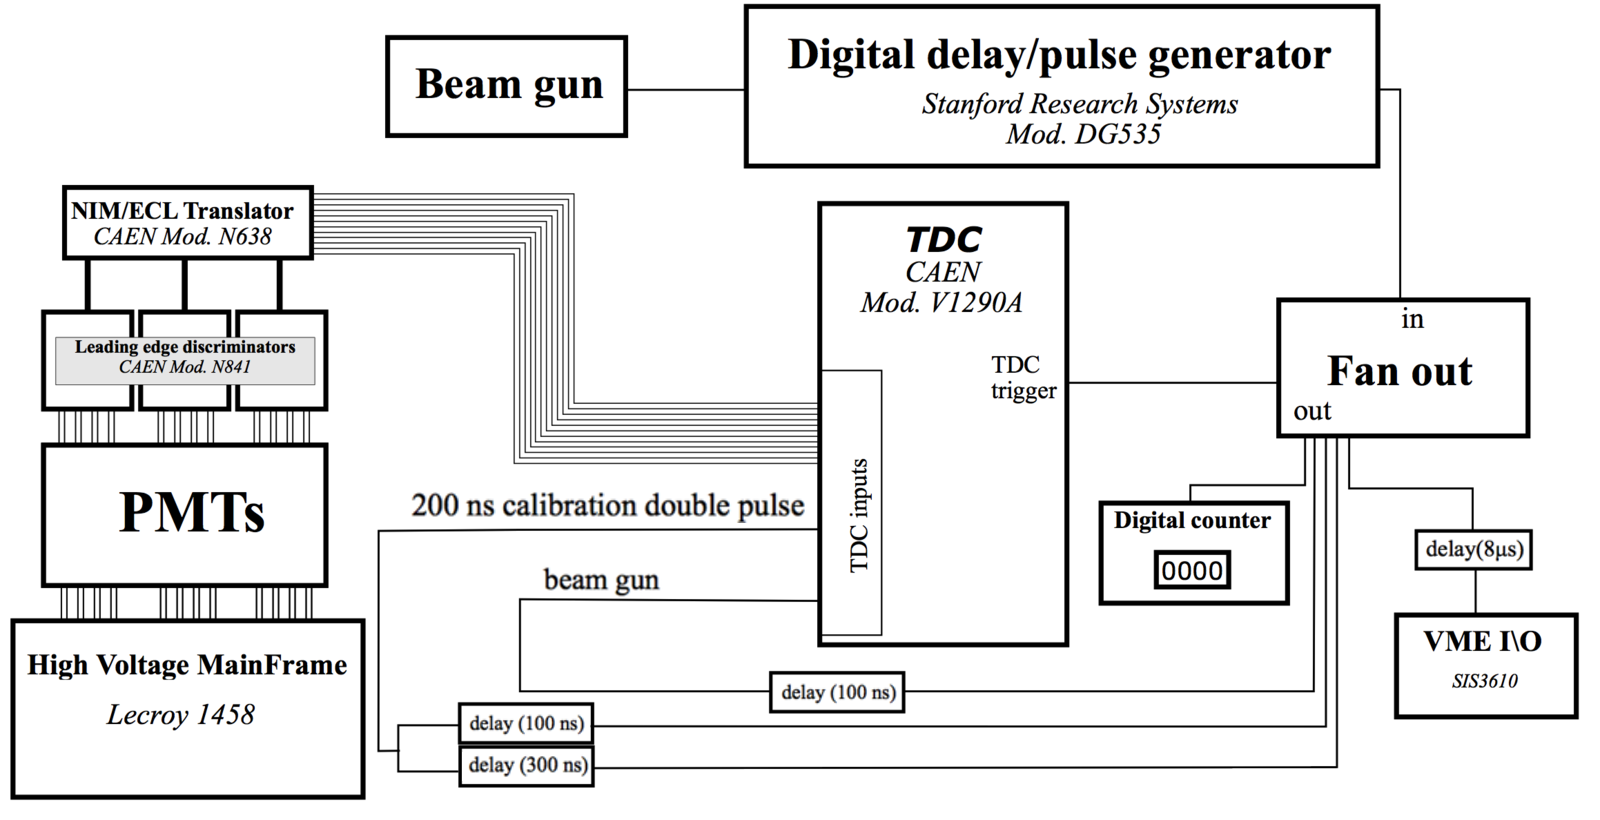
\includegraphics[width=\textwidth]{Content/Methods/WiringDiagram.png}
\caption{Wiring diagram of the entire electronics setup. }
\label{fig:WiringDiagram}
\end{figure}